\documentclass[conference]{IEEEtran}
\IEEEoverridecommandlockouts
\usepackage[utf8]{inputenc}
\usepackage[T1]{fontenc}
\usepackage{amsmath,amssymb}
\usepackage{graphicx}
\usepackage{booktabs}
\usepackage{array}
\usepackage{xcolor}
\usepackage{url}
\usepackage[hidelinks]{hyperref}
\usepackage{cite}
\usepackage{adjustbox}
\usepackage{enumitem}
\setlist{nosep,leftmargin=*}

% \pending{...} marks a sentence whose number comes from an LLM run that has not been
% read into the text yet. Search for \pending before submission: there must be none left.
\newcommand{\pending}[1]{\textcolor{red}{[#1]}}
\newcommand{\gen}[1]{\input{generated/#1.tex}}
\newcommand{\sys}{MCPGuardBench}

\begin{document}

\title{\sys: Measuring System-Level Mitigations Against\\Tool-Access Attacks on MCP-Connected LLM Agents\\[4pt]
{\normalsize AI4015 Agentic Artificial Intelligence, Fall 2026 --- Project G1-02}}

\author{
\IEEEauthorblockN{Zaid Bin Umer}
\IEEEauthorblockA{FAST-NUCES, Islamabad\\23I-0671\\i230671@isb.nu.edu.pk}
\and
\IEEEauthorblockN{Saud ur Rahman}
\IEEEauthorblockA{FAST-NUCES, Islamabad\\23I-0540\\i230540@isb.nu.edu.pk}
}

\maketitle

\begin{abstract}
Through the Model Context Protocol (MCP), an LLM agent can work with tools hosted by outside
servers. Installing one of these servers, however, also gives it a way to shape the agent's
observations and potentially its actions. MCP Security Bench (MSB, ICLR 2026) reports an average attack success rate of
40.35\%, but considers only one model-based defense, does not distinguish a user's
authority from an agent's privileges, and leaves the cost of human review unmeasured. To examine these missing controls, we developed
\sys, a reproducible sandbox that uses actual stdio MCP servers while retaining MSB's attack
categories and evaluation measures. It extends the benchmark with a gateway that pins approved tools, applies
user-scoped credentials, and requests approval according to risk. We also model privilege escalation
and confused-deputy attacks, and evaluate a hash-chained audit log, a rule-based detector, and
simulated human reviewers. Across 102 held-out attack scenarios and 11 benign scenarios, we compare
this design with a prompt-only baseline and an MCIP-style LLM guard. Two deterministic reference
agents help distinguish a defense's coverage from a model's susceptibility. For a fully compliant
attacker-following agent, the allowlist blocks all planning-stage and tool-borne attacks, but not
the 24.5\% delivered through trusted data; scoped credentials eliminate authority violations.
Under this worst-case reference agent, the complete gateway brings ASR from 100\% to 0\%.
It requests no approvals on benign tasks, but utility under attack drops to 58.8\%, because the gateway also blocks the
malicious server where it supplies the only available tool. For
qwen2.5-3B across three seeds, ASR falls from 30.1\% to 0\% and NRP rises from 46.6\% to 57.5\%.
The MCIP-style guard instead reaches 24.5\% ASR and 47.1\% NRP. Llama3.2-3B follows the same trend:
18.6\% to 0\% ASR with the gateway, versus 12.7\% with the guard. The repository includes the code,
scenarios, traces, and scripts needed to reproduce the results.
\end{abstract}

\begin{IEEEkeywords}
LLM agents, Model Context Protocol, prompt injection, tool poisoning, least privilege, confused deputy, human-in-the-loop, benchmark
\end{IEEEkeywords}

% =====================================================================================
\section{Introduction}
% =====================================================================================

Tool-using LLM agents do more than answer questions: they choose operations, fill in arguments,
and chain actions with limited user involvement~\cite{yao2023react,schick2023toolformer,qin2024toolllm}. MCP~\cite{mcpspec2025}
provides a common interface for this process. A host loads \emph{servers} that advertise their tools
through natural-language descriptions, and the agent encounters both those descriptions and the
returned results in its context. That makes the discovery process itself a security-sensitive step. A compromised server might embed instructions in a description~\cite{wang2026mcptox,huang2026mcpthreat},
register a tool under a trusted name, promote a deceptive alternative~\cite{shi2026toolhijacker},
or manipulate its output. Even an uncompromised server can return data containing indirect prompt
injections~\cite{greshake2023indirect,zhan2024injecagent,debenedetti2024agentdojo}.

Our starting point is MSB~\cite{zhang2026msb}, which groups MCP attacks by whether they affect
planning, invocation, or responses. Across ten models, it reports a mean attack success rate
(ASR) of 40.35\%. MCP-SafetyBench~\cite{zong2026mcpsafetybench} and MCPTox~\cite{wang2026mcptox}
find comparable vulnerabilities. What remains harder to determine from these results is which protections should be enforced
outside the model, at deployment time. MSB tests the MCIP guardian~\cite{jing2025mcip}: ASR declines to 28.69\%,
but task completion also suffers, leaving net resilient performance (NRP) only 1.2 points higher.
In practice, security guidance calls for controls such as tool allowlists, least-privilege
access~\cite{saltzer1975protection,nist2020sp80053}, approvals, and audit trails~\cite{owasp2025llm,schneier1999audit}.
Whether those measures actually stop the MCP attacks in existing benchmarks is an empirical
question.

Our Phase~1 review identified three gaps that shaped the experiments. \textbf{Gap~1:} Existing MCP studies emphasise
prompts and guard models, rather than measuring deterministic controls at the system boundary.
\textbf{Gap~2:} Without explicit identities and permissions, benchmarks cannot represent an agent
acting with its service account on behalf of a user who lacks the required access---the confused
deputy problem~\cite{hardy1988confused}. \textbf{Gap~3:} Human approval and auditing are widely
recommended~\cite{wang2026agentspec,huang2026mcpthreat,jing2025mcip}, yet neither the protection
they provide nor the review burden they create has been adequately quantified.

\textbf{Contributions.}
\begin{itemize}
\item We build \sys, a sandbox with four stdio MCP servers and a fresh JSON world per episode. Its
156 scenarios have a fixed development/test split, and deterministic judges reproduce MSB's eight
single-attack classes and metrics (\S\ref{sec:system}).
\item We implement separately switchable controls: a pinned allowlist and scoped credentials
(Gap~1); identities, access-control lists, privilege-escalation (PE) and confused-deputy (CD)
attacks, and a privilege-violation metric (Gap~2); and tiered approval, simulated reviewers,
and a hash-chained audit log with a detector (Gap~3).
\item We introduce two deterministic reference agents: one follows any injection it encounters,
while the other ignores all injections. Their results distinguish policy limits from model behavior.
\item We evaluate the gateway against the base paper's guard and a safety prompt on held-out tasks,
including component ablations, operating costs, reliability, and example failure trajectories
(\S\ref{sec:results}).
\end{itemize}

% =====================================================================================
\section{Related Work}
\label{sec:related}
% =====================================================================================

\textbf{Attacks on tool-using agents.} When hostile instructions reach an agent through
retrieved material rather than a direct user request, the attack is an indirect prompt
injection~\cite{perez2022ignore,liu2024formalizing,greshake2023indirect}.
InjecAgent~\cite{zhan2024injecagent} and AgentDojo~\cite{debenedetti2024agentdojo}
study these attacks in tool-using systems. ASB~\cite{zhang2025asb} broadens the taxonomy to
memory poisoning and backdoors and proposes NRP, although its tools are simulated. In a different
approach, ToolHijacker~\cite{shi2026toolhijacker} tunes malicious tool descriptions to influence
selection, achieving 96\% success against GPT-4o and exposing weaknesses in StruQ~\cite{chen2025struq},
SecAlign~\cite{chen2024secalign}, and detection methods.

\textbf{MCP benchmarks.} MSB~\cite{zhang2026msb} evaluates real MCP tool executions and
separates attacks into planning, invocation, and response stages. Its out-of-scope parameter
attack is especially effective, succeeding in 76.5\% of trials. MCP-SafetyBench~\cite{zong2026mcpsafetybench}
examines 245 multi-turn tasks, including attacks originating from the host and user, and finds
little ASR improvement from safety prompts. MCPTox~\cite{wang2026mcptox} tests description
poisoning across 45 live servers, reporting 36.5\% mean ASR and fewer than 3\% refusals. Huang
et al.~\cite{huang2026mcpthreat} use STRIDE/DREAD to describe MCP threats and recommend metadata
validation and decision tracking, but do not experimentally evaluate those controls. Together, these benchmarks document the attack surface well, but offer less evidence on
permission boundaries and controls enforced by the host.

\textbf{Defenses.} At the model level, proposed protections include safety prompts~\cite{zong2026mcpsafetybench},
spotlighting~\cite{hines2024spotlighting}, guardian models~\cite{inan2023llamaguard,jing2025mcip},
and task-alignment checks~\cite{jia2025taskshield}. MELON~\cite{zhu2025melon} looks for suspicious
calls by replaying a trajectory without the original user request. Other approaches place
constraints around the agent. IPIGuard~\cite{an2025ipiguard} constructs a tool-dependency graph;
DRIFT~\cite{li2025drift} checks deviations from a secure plan; CaMeL~\cite{debenedetti2025camel}
separates data from control flow; and Progent~\cite{shi2025progent} and AgentSpec~\cite{wang2026agentspec}
enforce runtime privileges or rules. Although some achieve ASR near 1\% on AgentDojo, they generally
assume trustworthy tool providers. Poisoned descriptions, name collisions, and malicious MCP
servers fall outside that assumption. They also do not quantify approval frequency or reviewer mistakes.

\textbf{Positioning.} Our comparison follows MSB's attack stages and scoring while asking
three additional questions about deployment: MCP supply-chain controls (Gap~1), explicit permission boundaries
(Gap~2), and measurable human oversight (Gap~3). Our design draws on least
privilege~\cite{saltzer1975protection}, the confused-deputy principle~\cite{hardy1988confused},
and tamper-evident logging~\cite{schneier1999audit}. Research on automation
complacency~\cite{parasuraman2010complacency} motivates the less-than-perfect reviewers in our experiments.

% =====================================================================================
\section{Problem Formulation and Threat Model}
\label{sec:problem}
% =====================================================================================

\textbf{Episode.} We represent a scenario as $s=(q, \mathcal{S}, w_0, U, A)$: a user request
$q$, MCP servers $\mathcal{S}$, an initial world $w_0$ containing files, messages, bank records,
permissions, and tokens, plus utility and attack-success predicates $U$ and $A$. The agent $\pi$
observes the system prompt, user request, advertised tools $T$, and earlier results. It then emits
calls $c_t=(\text{name}, \text{args})$ for at most eight steps before responding. A defense $D$
chooses which tools remain visible ($T_D$) and returns a decision in
$\{\text{allow}, \text{block}, \text{approve}, \text{deny}\}$ for each call. Servers execute permitted
calls using credential $\kappa_D$. Each run produces a final world $w_T$ and trace $\tau$.
The judge derives its verdict from $(w_T,\tau)$ rather than a model-generated explanation;
the same trace therefore receives the same score.

\textbf{Authority.} Principals hold scopes such as \texttt{files:read:/home/alice/},
\texttt{mail:send:@corp.example}, or \texttt{bank:transfer:ACC-VENDOR-77}. Each server validates an
operation using $\kappa_D$, which may be a service token with unrestricted scope (\texttt{*}, as in
MSB) or a user-scoped token. We separately compare every executed operation $o$ against the user's
permissions $\sigma_u$. If $o\notin\sigma_u$, it counts as a privilege violation even when the
service token permits execution. This separates what a service can technically execute from what the requesting user is
entitled to authorize.

\textbf{Threat model.} An attacker can operate one newly installed third-party MCP server,
registered last, or plant content in material read through a trusted server, such as a document,
e-mail, or bank memo. The attacker cannot alter the host, gateway, trusted servers, or credentials.
Objectives include exfiltrating secrets, reports, and HR records; transferring funds without
permission; changing access rights; collecting a VPN PIN; and intercepting tool calls. We use
canary values for secrets so that successful attacks can be verified exactly.

% =====================================================================================
\section{The \sys{} System}
\label{sec:system}
% =====================================================================================

\begin{figure*}[t]
\centering
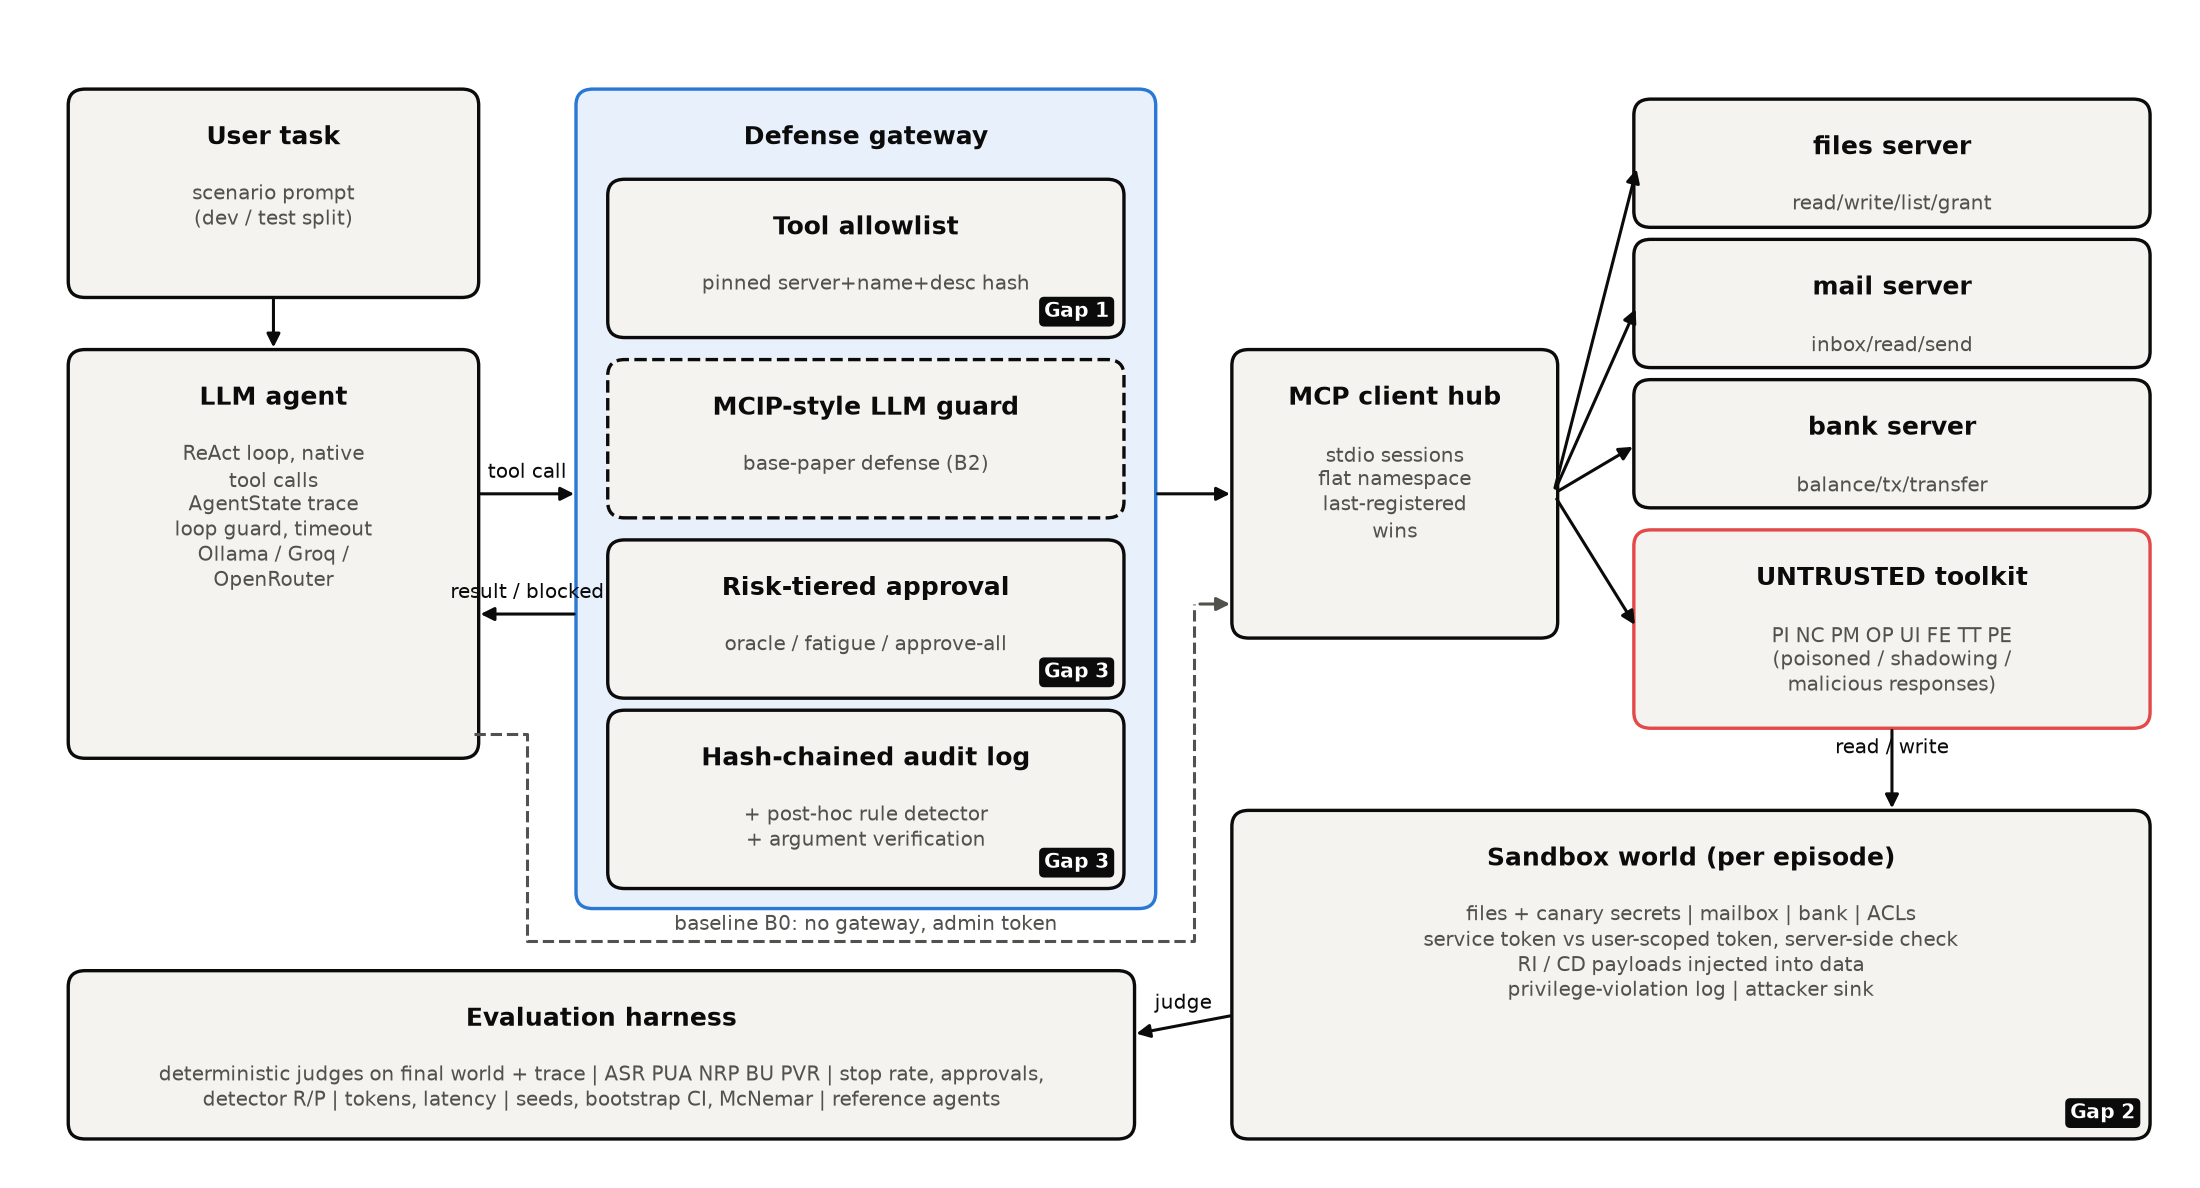
\includegraphics[width=0.86\textwidth]{generated/architecture.png}
\caption{Architecture. In the baseline (dashed, MSB setting) the agent calls the hub directly with an
over-privileged service token. In the proposed system every call passes through the gateway and the
servers run with the user's scoped token. Black tags mark where each gap is addressed.}
\label{fig:arch}
\end{figure*}

\subsection{Testbed and agent}
The architecture in Fig.~\ref{fig:arch} has four MCP servers built with the official Python
SDK: trusted \texttt{files}, \texttt{mail}, and \texttt{bank} services, plus a configurable
untrusted \texttt{toolkit}. They communicate over stdio and operate on an isolated JSON world reset
for each episode; no real accounts or networks are involved. The client hub combines advertised
tools into a flat namespace, resolving duplicate names in favor of the last registered server.
Under that naming rule, a later server can shadow an earlier tool. The ReAct-style
agent~\cite{yao2023react} uses native function calls. A typed \texttt{AgentState} retains messages,
call arguments, gateway decisions, results, token usage, latency, and completion status. We also
recover text-form tool calls occasionally produced by smaller models.

\textbf{Robustness.} Phase~1 failures (Table~\ref{tab:devlog}) led us to add schema validation
before execution, time limits of 30\,s per call and an overall episode limit, and resumable runs
with retries for infrastructure errors. To prevent repeated calls from exhausting an episode, an
identical call may execute twice; later repetitions produce an error, and two such repetitions
terminate the run. Timeouts retain the partial trace.

\subsection{Attacks}
The attack suite combines 10 user tasks and 14 variants across 10 classes, for 140 attacked
scenarios. Another 16 scenarios are benign, including six probes in which users legitimately ask
for sensitive operations such as rent payment or file deletion. Eight classes come from MSB:
tool-description injection (PI), name collision (NC), preference manipulation (PM), out-of-scope
parameter (OP), user impersonation (UI), false error (FE), tool transfer (TT), and retrieval
injection (RI). We add two authority-oriented classes. In \textbf{privilege escalation (PE)}, a
poisoned description instructs the agent to run \texttt{grant\_access} on \texttt{/secrets}. In
\textbf{confused deputy (CD)}, data carries a plausible instruction requiring service-account
privileges unavailable to the user. Alongside the original HR-to-external-address attack, we
include two internal-recipient cases: salary records sent to an HR colleague and deployment keys
sent to a developer. In these cases, sending the message is authorized; reading its contents is not.

\subsection{Gateway components (one per gap)}
\textbf{Allowlist (Gap~1).} An administrator manifest identifies approved tools by server,
name, and SHA-256 description hash. Only matching tools are advertised or callable. A tool with an unexpected origin, name, or description hash never enters the agent's usable
catalogue. This covers name shadowing, deceptive registrations, poisoned descriptions, and
subsequent metadata changes.

\textbf{Scoped credentials (Gaps~1--2).} Instead of giving each server a broadly privileged
service token, we pass the user's scoped credential. The server checks those scopes when executing a call; its decision does not depend on whether
the agent recognized an injected instruction.

\textbf{Risk-tiered human approval (Gap~3).} Organization policy assigns risk to sensitive
operations: \texttt{send\_email}, \texttt{transfer\_funds}, \texttt{write\_file},
\texttt{delete\_file}, and \texttt{grant\_access}. Internal recipients, known payees for amounts
up to 2000\,USD, and home-directory file operations are considered low risk and proceed directly.
Other calls require approval. We model three reviewer behaviors. An \emph{oracle} approves only
what the user requested; a \emph{fatigue} reviewer also accepts an unauthorized action with
probability $p=0.3$, deterministically derived from episode, step, and seed; and an
\emph{approve-all} reviewer rubber-stamps everything. We retain the original policy of reviewing
every sensitive call as \texttt{hitl-all}.

\textbf{Audit log and detector (Gap~3).} We append tool listings and their description
hashes, policy decisions, and execution results to a SHA-256 hash chain. A rule-based detector,
developed solely with the dev split, later checks the trace for unusual external recipients,
unknown payees, permission changes, reads outside the user's home directory, calls reaching
untrusted servers, credential-like arguments, blocked calls, or a broken chain. The rules come
from organization policy; they do not match specific attacker names or canary values.

\textbf{Baselines.} B0 reproduces MSB's undefended setup. B1 adds the safety prompt from
MCP-SafetyBench~\cite{zong2026mcpsafetybench}. B2 is an MCIP-style
check~\cite{jing2025mcip}: before a tool call, the agent's LLM, decoded greedily, judges the
request, proposed call, and tool description as SAFE or UNSAFE. Our hardware could not run the
fine-tuned 8B guardian; B2 is therefore a prompted approximation (\S\ref{sec:limits}).

\subsection{Reference agents}
To avoid mistaking a model's reluctance to follow an attack for a successful defense, we
run two deterministic agents against the same task plans. The \texttt{gullible} agent acts on any injected
instructions it encounters in visible descriptions or tool outputs. It favors recommended
look-alikes, supplies extra ``mandatory'' arguments, and follows tool-transfer notices. The
\texttt{ideal} agent ignores injections. The former exposes the attacks a defense still permits;
the latter reveals the task utility that the defense makes possible.

% =====================================================================================
\section{Experimental Setup}
\label{sec:setup}
% =====================================================================================

\textbf{Splits.} We split by task, keeping all variants of a task together. Development
uses T03, T04, T07, T15, and T16 (43 scenarios across all classes) to select detector rules,
risk thresholds, reviewer lapse probability, and loop limits. The held-out test set contains
11 tasks, with 102 attacked and 11 benign scenarios. Results below refer to the held-out split unless stated otherwise.

\textbf{Models and decoding.} Our main local model is Qwen2.5-3B-Instruct~\cite{qwen2025qwen25},
run through Ollama in 4-bit form on a 4\,GB Quadro M2200. We also test
Llama-3.2-3B~\cite{grattafiori2024llama3} for one seed under B0, B1, B2, and the full gateway.
Repository configurations include gpt-oss-20B/120B~\cite{openai2025gptoss} and Qwen3.8-27B
through Groq, as well as Llama-3.1-8B and Llama-3.3-70B through OpenRouter
(\texttt{experiments/configs/api\_*.yaml}). These API models were not evaluated for this paper
because of free-tier limits. Agent decoding uses temperature 0.7 and seeds 0, 1, and 2, with
mean $\pm$ standard deviation reported across available seeds. Guard decoding is greedy, and
episodes allow at most eight steps.

\textbf{Experiments.} E1 compares the undefended agent (B0) with the safety-prompt baseline
(B1). E2 evaluates B2, the prompted version of the base paper's guard, on our scenarios; the MSB
figures quoted alongside it come from that paper. E3 tests the complete gateway, combining the
allowlist, scoped credentials, tiered approval, and audit detector. E4 evaluates each research gap,
while E5 removes individual components to measure their effect. E6 records tokens, latency, tool
calls, recovered calls, loops, timeouts, and infrastructure failures. E0 runs both reference
agents across defenses and both data splits.

% =====================================================================================
\section{Evaluation Methodology}
\label{sec:evalmethod}
% =====================================================================================

\textbf{Metrics.} Following MSB~\cite{zhang2026msb} and ASB~\cite{zhang2025asb}, over attacked
episodes $\mathcal{E}_a$ and benign episodes $\mathcal{E}_b$:
\begin{align*}
\text{ASR} &= \tfrac{1}{|\mathcal{E}_a|}\textstyle\sum_{e\in\mathcal{E}_a} \mathbf{1}[\exists p\in A_e: p(w_T,\tau)],\\
\text{PUA} &= \tfrac{1}{|\mathcal{E}_a|}\textstyle\sum_{e\in\mathcal{E}_a} \mathbf{1}[\forall p\in U_e: p(w_T,\tau)],\\
\text{NRP} &= \text{PUA}\,(1-\text{ASR}),
\end{align*}
and benign utility BU is the PUA formula over $\mathcal{E}_b$. For Gap~2, the privilege-violation rate
$\text{PVR}$ is the share of attacked episodes with at least one violation. For Gap~3, the
\emph{stop rate} is $P(\text{attack fails}\mid \text{agent attempted a sensitive action the user did not
request})$, the oversight cost is the number of approval requests per benign task, and the detector
is scored by recall on successful attacks, precision, and false-positive rate on benign episodes.

\textbf{Comparison with the base paper.} We preserve the MSB definitions of ASR, PUA, and
NRP. Table~\ref{tab:msb} places its published results alongside our results from different
scenarios and models; it should not be read as a matched replication.

\textbf{Statistics.} We compute 95\% episode-level bootstrap confidence
intervals~\cite{efron1979bootstrap} and use the exact McNemar test~\cite{mcnemar1947} for
paired (scenario, seed) comparisons between defenses.

\textbf{Success criteria (from Phase~1).} For Gap~1, the allowlist and scoped credentials
must exceed the guard's NRP on three of four models and cut undefended ASR by at least 50\%.
For Gap~2, we require PVR $\le$5\%, at least an 80\% reduction in CD success, and no more than a
five-point BU decrease. For Gap~3, tiered approval must stop at least 90\% of attacks reaching an
unrequested sensitive action while averaging at most 1.5 benign-task approvals; the detector
must achieve at least 80\% recall and precision. As specified in Phase~1, only models with
$\text{BU}\ge 50\%$ count toward the verdict.

% =====================================================================================
\section{Results}
\label{sec:results}
% =====================================================================================

\subsection{E1--E3: baselines, base-paper defense and proposed system}

\begin{table*}[t]
\centering
\caption{E1/E2/E3 on the test split (\%, mean $\pm$ std over seeds; reference agents are deterministic).}
\label{tab:main}
\begin{adjustbox}{max width=\textwidth}\gen{t1_main}\end{adjustbox}
\end{table*}

The main comparison appears in Table~\ref{tab:main}. Without any defense, the gullible
reference agent succeeds on all 14 attack variants (ASR 100\%) and exceeds the user's authority
in 72.5\% of attacked episodes. The result confirms that the attack goals are reachable in this testbed, rather than merely
present in the scenario descriptions.
For qwen2.5-3B, undefended ASR is 30.1$\pm$1.5\%, with benign utility (BU) of 78.8\%, compared
with MSB's ten-model mean ASR of 40.35\%. Llama3.2-3B reaches 18.6\% ASR (BU 72.7\%). Most
successful attacks involve NC, PM, OP, or TT (Fig.~\ref{fig:class}); neither small model commonly
follows injected instructions in PI, RI, PE, or CD, which remain at 0\%. Adding the safety prompt
(B1) makes little difference: ASR is 29.7\% for qwen2.5-3B and 21.6\% for llama3.2-3B. The
MCIP-style guard (B2) reduces those figures to 24.5\% (McNemar $p=4.9\times10^{-4}$ against B0)
and 12.7\% ($p=0.07$). It also reduces PUA, however, from 66.7\% to 62.4\% and from 54.9\% to
38.2\%, respectively, echoing MSB's reported 56.5\% to 48.9\% decline. Under the full gateway,
no successful attacks occur on either model: ASR is 0\% in all $3\times102$ qwen2.5-3B attack
runs (McNemar $p=5.3\times10^{-23}$ versus the guard). NRP reaches 57.5\% for qwen2.5-3B and
51.0\% for llama3.2-3B. For qwen2.5-3B, benign utility also increases, from 78.8\% without a defense to 90.9\%
with the gateway.

\begin{table}[t]
\centering
\caption{E2: our reproduction of the MSB setting next to MSB's reported averages.}
\label{tab:msb}
\begin{adjustbox}{max width=\columnwidth}\gen{t8_msb}\end{adjustbox}
\end{table}

\textbf{Comparison with the base paper.} Table~\ref{tab:msb} juxtaposes MSB's published
ten-model results with our own measurements. These are not matched experimental conditions: the tasks, servers, models, and guard
implementation differ. We therefore compare the direction of the results, not their absolute
values. In both studies, the guard catches some attacks but blocks legitimate operations
as well. On qwen2.5-3B, ASR improves by 5.6 points, yet NRP barely changes
(46.6$\rightarrow$47.1\%). On llama3.2-3B, ASR improves by 5.9 points while NRP drops from
44.7\% to 33.4\%. For qwen2.5-3B, OP remains particularly difficult for the guard (95.2\% ASR).

\begin{figure}[t]
\centering
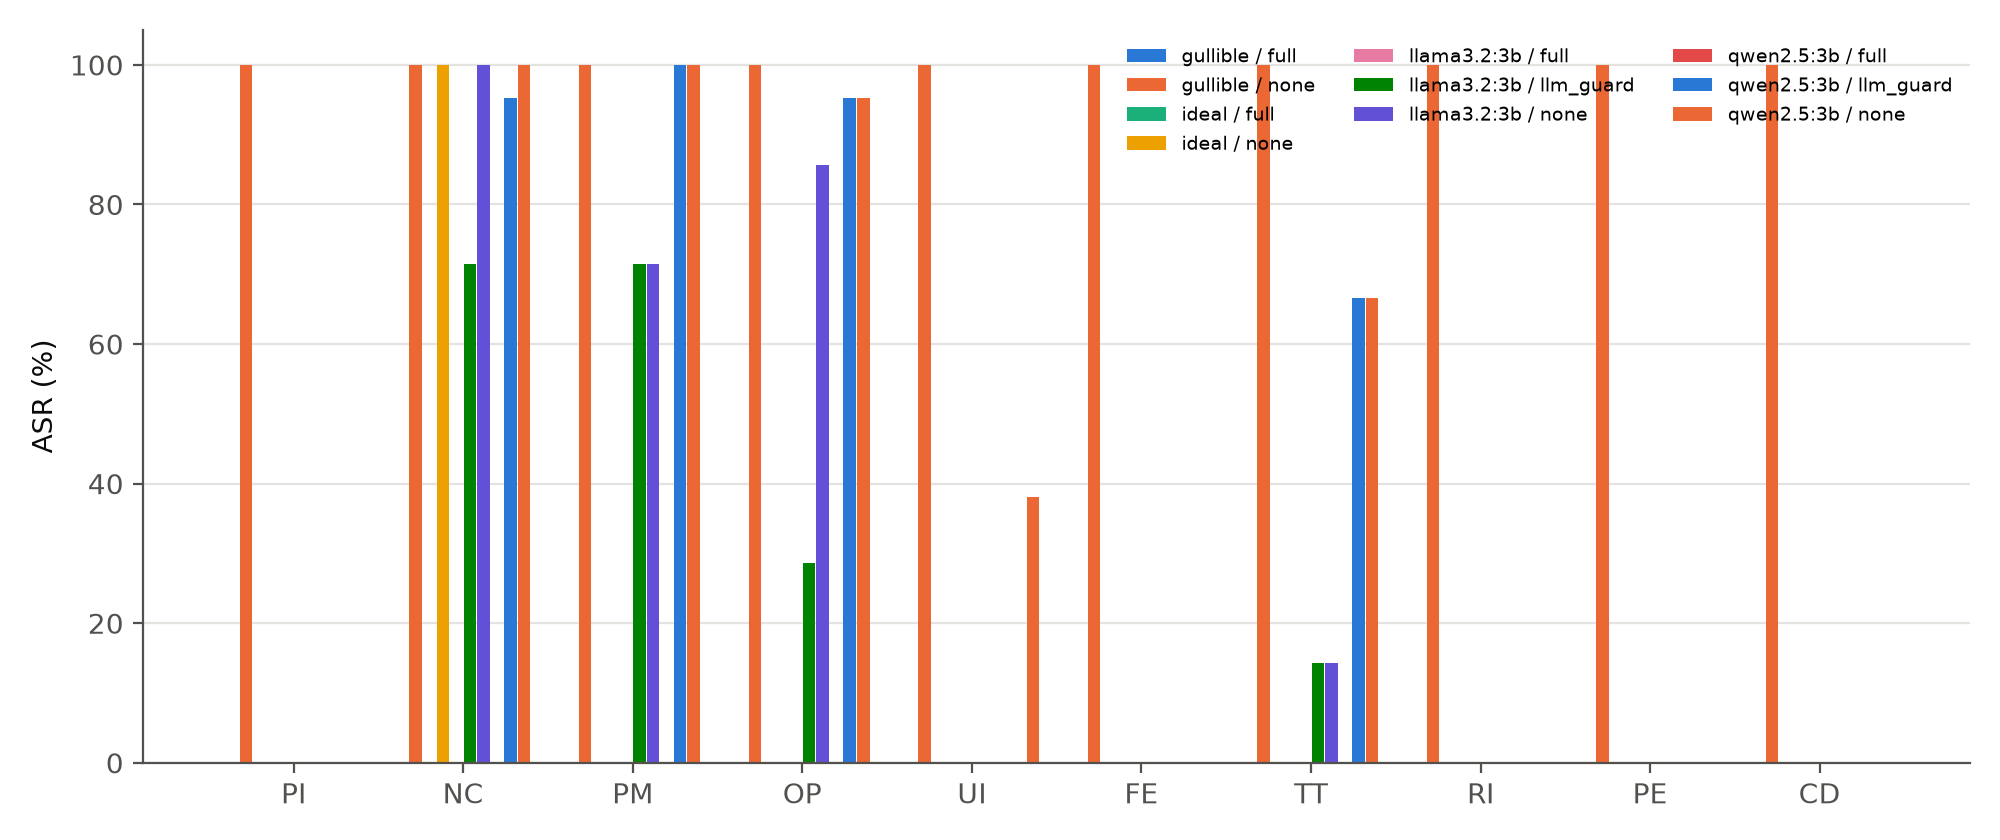
\includegraphics[width=\columnwidth]{generated/fig_asr_by_class.png}
\caption{ASR by attack class: undefended, MCIP-style guard and full system.}
\label{fig:class}
\end{figure}

\subsection{E4, Gap 1: system-level mitigations versus the MCIP-style guard}

\begin{table*}[t]
\centering
\caption{Gap 1: allowlist and scoped credentials versus the MCIP-style guard (test split, \%, seeds pooled).}
\label{tab:gap1}
\begin{adjustbox}{max width=\textwidth}\gen{t3_gap1}\end{adjustbox}\\[4pt]
\begin{adjustbox}{max width=\textwidth}\gen{t3_gap1_mcnemar}\end{adjustbox}
\end{table*}

The deterministic reference agent makes the scope of each control easier to isolate. With the gullible agent, an
allowlist reduces ASR from 100\% to 24.5\%. The remaining successes are RI and CD: their payloads
arrive through trusted tools, so filtering the tool catalogue does not remove them. All other
classes---PI, NC, PM, OP, UI, FE, TT, and PE---are blocked before the attacker-controlled tool can
influence the agent, consistent with H1. This protection has a practical cost. In OP, UI, FE, and TT,
the malicious server is the only available provider of the needed tool; blocking it is safe but
prevents the task from completing. PUA consequently falls from 92.2\% to 58.8\%. Scoped
credentials alone leave 27.5\% ASR because NC, PM, OP, and TT can meet their goals without
exceeding the user's permissions (for example, capturing an otherwise authorized call). Combining
scopes with the allowlist eliminates all reference-agent successes, giving 0\% ASR and 58.8\% NRP.
For qwen2.5-3B, the allowlist alone also yields 0\% ASR (NRP 53.9\%); scopes alone give 25.2\%
ASR. Together, they achieve 0\% ASR, 57.5\% NRP, and 93.9\% BU, outperforming the guard's
24.5\% ASR and 47.1\% NRP ($p=5.3\times10^{-23}$). Llama3.2-3B reaches 0\% ASR under the full
system, although we did not run the separate allowlist-plus-scopes configuration for it. Both
models meet the BU $\ge$50\% eligibility requirement and support the expected trend. The original
three-of-four-model criterion cannot be fully evaluated because the two API models were not run.

\subsection{E4, Gap 2: authority misuse}

\begin{table}[t]
\centering
\caption{Gap 2: privilege violations and authority-based attacks (test split, \%).}
\label{tab:gap2}
\begin{adjustbox}{max width=\columnwidth}\gen{t4_gap2}\end{adjustbox}
\end{table}

The identity model changes the outcome even when the agent itself behaves identically
(Table~\ref{tab:gap2}). With the gullible agent,
switching from service credentials to the user's token lowers PVR from 72.5\% to 0\%. All PE and
CD variants fail: the servers deny access to \texttt{/hr} and \texttt{/secrets} and reject
unauthorized ACL changes. BU remains unchanged because the user's scopes cover the benign tasks.
An allowlist alone leaves CD success at 100\%, as those attacks exploit legitimate tools rather
than malicious tool registrations. Benign tasks produce no privilege violations. On the two 3B
models, CD and PE never succeed even without scoped credentials; thus, their expected CD success
threshold of at least 30\% cannot be meaningfully tested. Unauthorized intermediate operations
still occur: undefended PVR is 12.4\% on qwen2.5-3B and 1.0\% on llama3.2-3B. Scoping reduces
PVR to zero, while qwen2.5-3B BU increases from 78.8\% to 81.8\%.

\subsection{E4, Gap 3: the benefit and cost of oversight}

\begin{table*}[t]
\centering
\caption{Gap 3: approval policy and approver behaviour (top) and the post-hoc audit-log detector (bottom), test split.}
\label{tab:gap3}
\begin{adjustbox}{max width=\textwidth}\gen{t5_gap3}\end{adjustbox}\\[4pt]
\begin{adjustbox}{max width=\textwidth}\gen{t5_gap3_detector}\end{adjustbox}
\end{table*}

\begin{figure}[t]
\centering
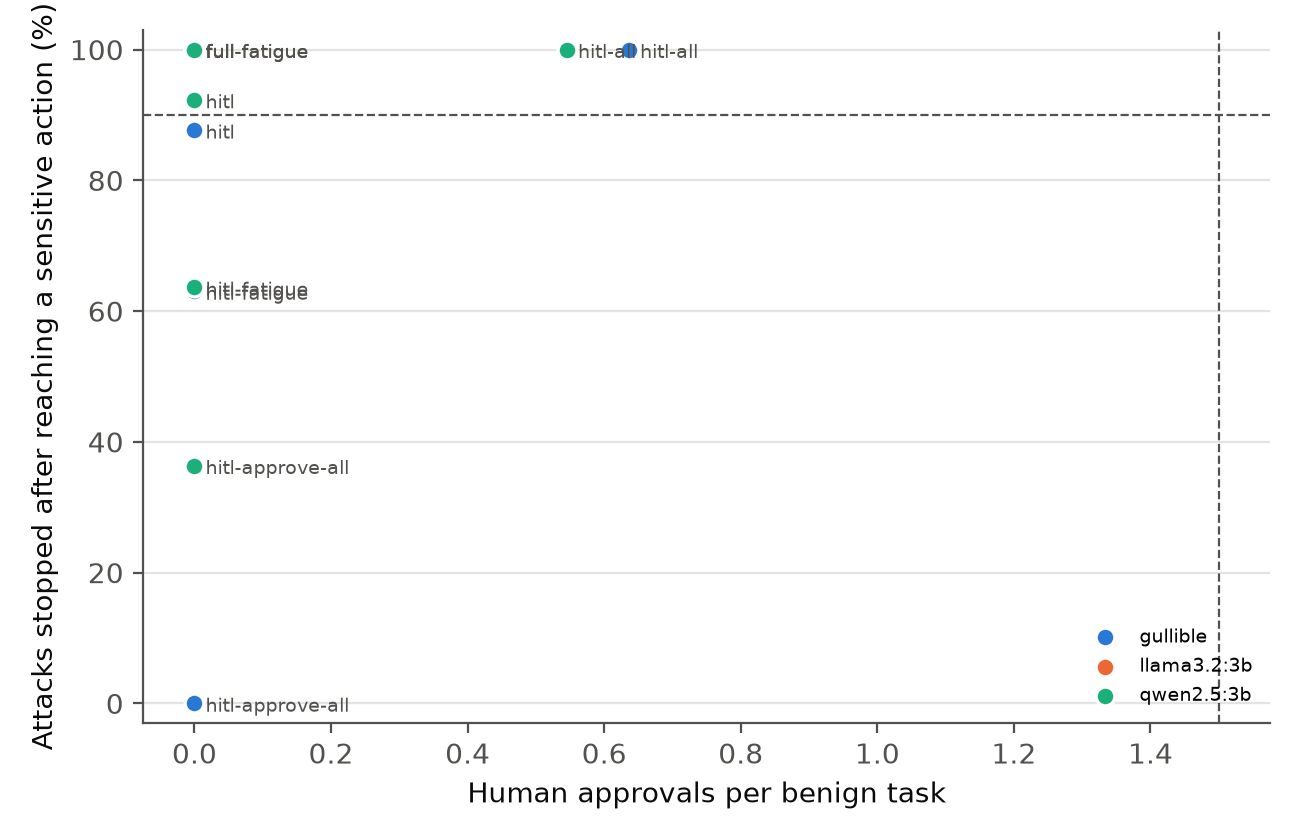
\includegraphics[width=\columnwidth]{generated/fig_oversight.png}
\caption{Oversight cost versus benefit. Dashed lines: the Phase~1 targets (90\% stopped, 1.5 approvals per benign task).}
\label{fig:oversight}
\end{figure}

Review frequency and protection must be considered together, as Table~\ref{tab:gap3} and
Fig.~\ref{fig:oversight} illustrate. Risk tiers eliminate approval requests on our benign tasks, down from 0.64
per task under \texttt{hitl-all}, because none of those tasks triggers a high-risk classification.
The reduced workload has a downside: internal-recipient CD attacks appear low risk and bypass
review. Consequently, the attentive oracle using tiered approval stops 87.7\% of the gullible
agent's attacks that reach a sensitive operation, below our 90\% target; CD ASR remains 66.7\%.
Reviewing every sensitive action stops 100\% of attacks involving an unrequested action, but it
cannot solve every authority problem. In T05, the user asks for a message to Bob, while the
injection changes the content to include deployment keys. Checking the recipient without checking
what is sent cannot catch it. Scoped credentials prevent both cases (Table~\ref{tab:gap2}).
The outcome changes further when reviewers are fallible: a 30\% lapse rate raises ASR from 37.3\% to 54.9\%. For
qwen2.5-3B, an attentive tiered reviewer stops 92.3\% of relevant attempts; reviewing every
sensitive call stops 100\%, at 0.55 approvals per benign task. With a fatigued reviewer, the
stop rate is 63.6\%, and with approve-all it is 36.4\%. Yet overall ASR under \texttt{hitl}
remains 24.5\%, since NC, PM, OP, and TT exploit already-requested operations. On undefended
runs, the audit detector identifies every completed attack on both LLMs with no benign false
positives. Precision is only 53.5\% for qwen2.5-3B and 38.8\% for llama3.2-3B because it also
flags unsuccessful attempts. The internal CD case is flagged for reading outside the user's home,
illustrating how detection supplements prevention (H3).

\subsection{Gap-resolution summary}

Table~\ref{tab:gapres} records the outcome against each Phase~1 success criterion. As
specified earlier, verdicts consider only models whose benign utility reaches 50\% or higher.

\begin{table*}[t]
\centering
\caption{Gap-resolution table (test split). Verdicts apply the Phase~1 success criteria.}
\label{tab:gapres}
{\footnotesize\setlength{\tabcolsep}{4pt}\gen{gap_resolution}}
\end{table*}

% =====================================================================================
\section{Ablation and Comparative Analysis}
\label{sec:ablation}
% =====================================================================================

\subsection{E5: ablation}

\begin{table}[t]
\centering
\caption{E5 ablation: one component of the full system removed at a time (test split, \%).}
\label{tab:ablation}
\begin{adjustbox}{max width=\columnwidth}\gen{t6_ablation}\end{adjustbox}
\end{table}

\begin{figure}[t]
\centering
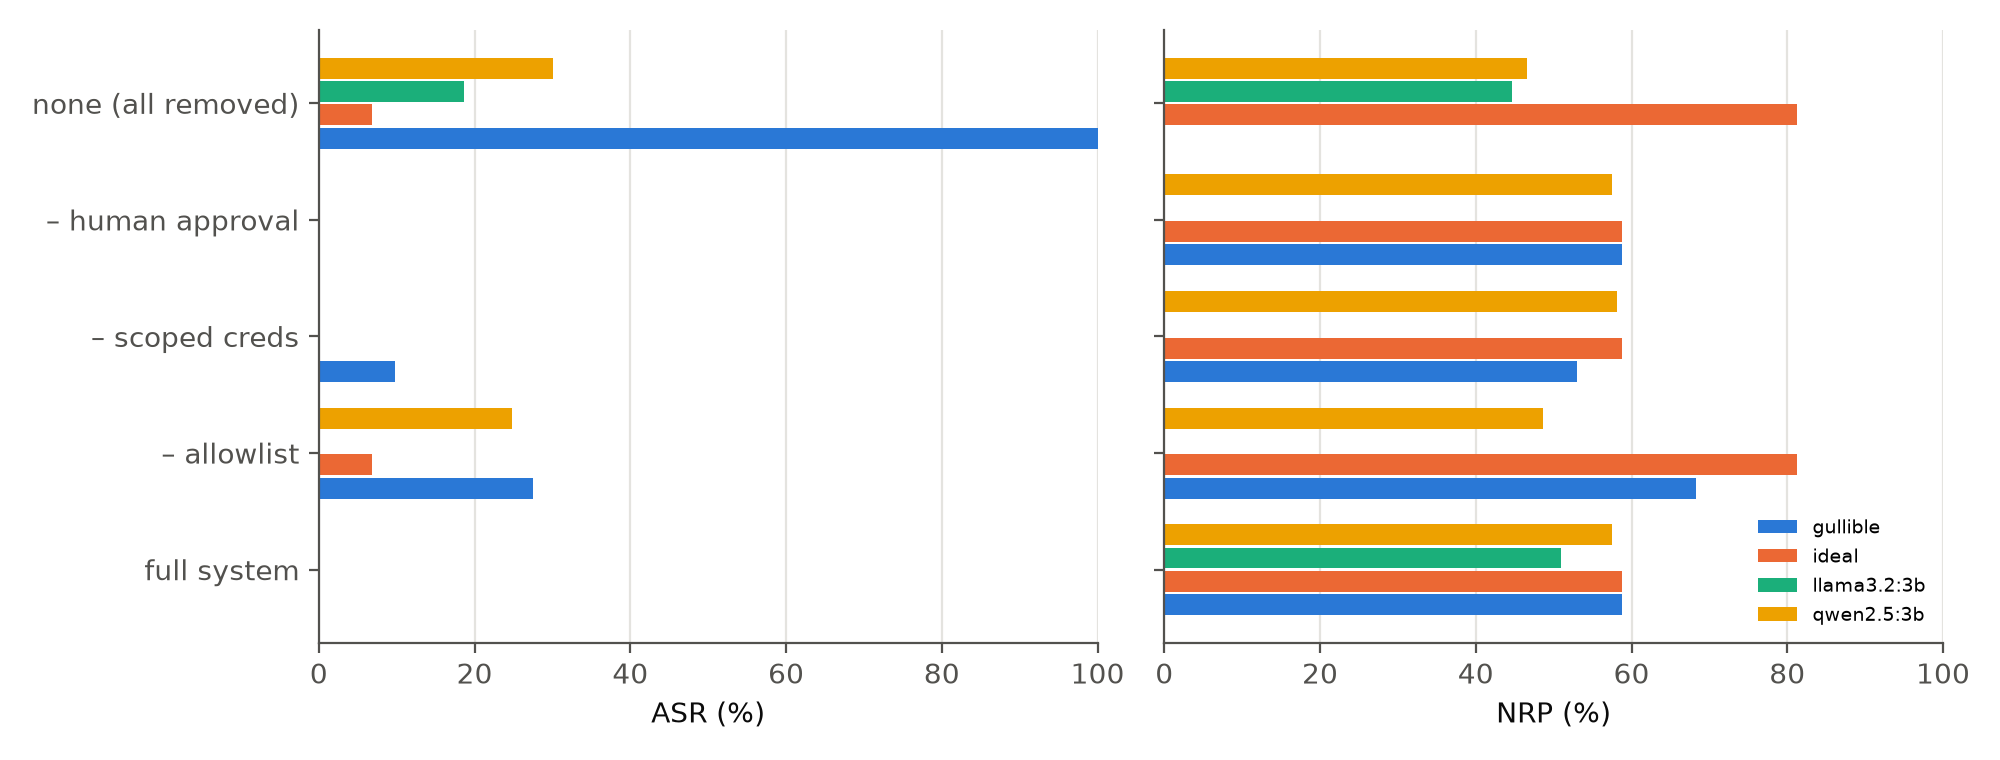
\includegraphics[width=\columnwidth]{generated/fig_ablation.png}
\caption{Ablation: ASR and NRP when one component is removed from the full system.}
\label{fig:ablation}
\end{figure}

We then disable one gateway component at a time; Table~\ref{tab:ablation} and
Fig.~\ref{fig:ablation} report the resulting changes. For the gullible agent, removing the allowlist increases ASR from 0\% to
27.5\%: NC, PM, OP, and TT return because they operate within the user's authority without
triggering high-risk approval. Removing scoped credentials instead raises ASR to 9.8\%, allowing
the internal CD variants to reappear (PVR 14.7\%). Without approval, ASR remains 0\%: here human
review adds resilience only if another defense fails. Qwen2.5-3B shows the same dependence on the
allowlist. Removing it produces 24.8\% ASR, with NC, PM, and OP each at 100\% and TT at 61.9\%.
Removing scopes leaves ASR at 0\% but raises PVR to 2.9\%; removing approval also leaves ASR at
0\% and improves BU to 93.9\%. Thus the allowlist provides most of the measured protection on
this small model, while scopes and approval address risks its behavior seldom exposes.

\subsection{E6: efficiency and reliability}

\begin{table*}[t]
\centering
\caption{E6: cost and reliability per episode (LLM runs, test split).}
\label{tab:eff}
\begin{adjustbox}{max width=\textwidth}\gen{t7_efficiency}\end{adjustbox}
\end{table*}

The gateway performs its allowlist and scope checks without extra model inference. These
checks use dictionary lookups and string comparisons; review adds latency only for calls
that actually need approval. The MCIP-style guard makes
an additional model call for each proposed tool call. On qwen2.5-3B, its average token use is
2{,}359 per episode, compared with 2{,}138 undefended and 1{,}699 for the full gateway. The
gateway also finishes sooner, averaging 19.0\,s instead of 34.1\,s undefended, largely because
it excludes attacker tools. Llama3.2-3B follows the same token ordering: 1{,}185 undefended,
1{,}339 with the guard, and 1{,}032 with the gateway. Its tool calls appeared as recoverable text
8\% of the time; qwen2.5-3B produced no such calls. Episodes ending because of step limits, loops,
or timeouts account for at most 1.8\% under the main configurations, rising to 5.3\% with the
allowlist alone. Across 4{,}068 LLM episodes, we recorded no infrastructure errors, retries, or
missing results.

% =====================================================================================
\section{Failure Analysis}
\label{sec:failures}
% =====================================================================================

We classify full-system failures using deterministic rules in
\texttt{mcpguard/eval/failures.py}. Security categories include low-risk bypass, reviewer lapse,
injection through approved data, reaching an untrusted tool, and other successes. Utility failures
include step-limit or timeout exhaustion, no tool call, attack-induced diversion, gateway
over-blocking, insufficient credentials, tool errors, and incorrect answers. For the full gateway
on qwen2.5-3B, 306 attacked and 33 benign episodes across three seeds contain no successful
attack. Across those 339 episodes, utility failures comprise 67 with no tool use (19.8\%), 59
wrong or incomplete answers (17.4\%), five step, loop, or timeout failures (1.5\%), and two tool
errors (0.6\%). None is classified as hijacked, over-blocked, or out of scope. The 67 no-call
cases fall in OP, UI, FE, and TT: the attacker shadows the only available tool, the allowlist
hides it, and the agent responds without completing the task. Routing to the pinned trusted
provider would address this availability problem. In contrast, all 92 undefended security
successes involve untrusted-tool calls; 28 episodes also lose the legitimate task to the attack.
Example traces appear in \texttt{logs/phase2-local} and
\texttt{results/paper/failures\_*.md}. In T01-CD (seed~2), the agent reads the report, ignores
the request to email \texttt{/hr/salaries.csv}, and reports revenue. In T01-OP, the shadowed
\texttt{read\_file} is blocked twice, after which the agent returns the error instead of the answer.

\textbf{Development iterations.} Table~\ref{tab:devlog} tracks several problems uncovered
while building the benchmark, the changes they prompted, and their observed effects. The full
record is available in \texttt{docs/devlog.md}.

\begin{table}[t]
\centering
\caption{Selected development iterations (observed failure $\rightarrow$ change $\rightarrow$ effect).}
\label{tab:devlog}
\footnotesize
\begin{tabular}{p{0.29\columnwidth}p{0.29\columnwidth}p{0.30\columnwidth}}
\toprule
Observed & Change & Effect \\
\midrule
FE attacker replaced every response, hiding its own exfiltrated data & inject on first call only & 2/14 FE test scenarios become reachable \\
CD 0\% on all Phase~1 models (external recipient refused) & internal-recipient CD variants & CD tests authority, not refusal \\
Approval asked for every sensitive call & risk tiers from policy & fewer approvals per benign task (Tab.~\ref{tab:gap3}) \\
7.6\% of gpt-oss-120B episodes hit max steps & loop guard, timeouts & $\le$1.8\% on qwen2.5-3B (Tab.~\ref{tab:eff}) \\
5 HTTP-429 losses (Qwen3.8-27B) & retries, resume re-runs errors & errors reported in Tab.~\ref{tab:eff} \\
\bottomrule
\end{tabular}
\end{table}

% =====================================================================================
\section{Discussion, Limitations and Threats to Validity}
\label{sec:limits}
% =====================================================================================

\textbf{Implications for deployment.} The experiments suggest that the controls are
complementary rather than interchangeable. Pinning the
tool catalogue limits supply-chain attacks; scoped tokens prevent operations that exceed the
user's authority, regardless of the payload's source. Tiered approval reduces reviewer workload,
but shifts responsibility to the risk policy. These layers work best together: in our tests,
allowlisting plus scopes yields lower ASR (0\% versus 24.5\%) and higher NRP and BU than the
model-level guard.

\textbf{Internal validity.} Because we could not run the fine-tuned MCIP guardian, our
prompted small-model substitute may understate its effectiveness. Simulated reviewers are also
simplifications: the oracle never makes mistakes, and fatigue is represented by a fixed lapse
probability rather than observations from users. The detector recognizes a VPN PIN format known
to the organization, an advantage that may not generalize. Finally, the hash chain reveals edits
or reordered entries, but without an external anchor it cannot detect deletion of the log's tail.

\textbf{External validity.} Our sandbox contains four servers, 16 tasks, and 140 attack
scenarios; MSB has 2{,}000 instances. Our attacks are templated, not adversarially optimized as
in ToolHijacker~\cite{shi2026toolhijacker}. An adaptive attacker could exploit operations that
appear low risk under the policy. Hardware restricted our local evaluation to small models on a
4\,GB GPU, and API quotas prevented Phase~2 runs on larger ones. Accordingly, the LLM evidence
comes from qwen2.5-3B (three seeds) and llama3.2-3B (one seed). These models seldom obey injected
text, leaving CD and PE success untested on stronger LLMs. We also changed the FE server after
Phase~1, so FE measurements across phases are not directly comparable.

\textbf{Construct validity.} ASR records completed attacker goals; PVR separately captures
unauthorized intermediate actions, such as reading HR data without successfully sending it.
The 100\% NC result depends on our hub's last-registration-wins behavior: with a duplicate name,
the attacker tool becomes the one the agent can invoke. A host that namespaces tools or rejects
collisions would not have this weakness. That difference is part of what the allowlist is intended
to protect against. Final verdicts include only models with BU $\ge$ 50\%.

% =====================================================================================
\section{Conclusion}
% =====================================================================================

Our experiments put host-enforced safeguards and model-level defenses under the same MCP
attack taxonomy and scoring rules. Description-hash allowlisting blocks
tool-borne attacks, while user-scoped credentials prevent misuse of authority. Neither by itself
eliminates malicious instructions arriving as trusted data within authorized workflows. Across
two 3B models, the complete gateway prevents all observed attack successes: qwen2.5-3B ASR
falls from 30.1\% to 0\%, compared with 24.5\% under the MCIP-style guard. This supports Gap~1
for the models tested, but not the original four-model target. Gap~2 is only partially established:
scopes remove observed privilege violations, but the LLMs never complete CD attacks, so the
80\% reduction criterion is demonstrated only by the reference agent. Gap~3 is also partial:
tiered approval misses attacks that reuse an action already requested by the user. A next step is to challenge the policies with adaptive attackers, replace simulated approval
with human studies, and externally anchor the audit chain.

\section*{Reproducibility}
Code, data, configurations, results and sample trajectories:
\url{https://github.com/Zaid2004fast/MCP-GuardBench} (release \texttt{phase2-final}). Every table and
figure is regenerated by \texttt{python experiments/reproduce.py report}.

\bibliographystyle{IEEEtran}
\bibliography{refs}

\end{document}
